%%%%%%%%%%%%%%%%%%%%%%%%%%%%%%%%%%%%%%%%%%%%%%%%%%%%%%%%%%%%%%%%%%%%
%% I, the copyright holder of this work, release this work into the
%% public domain. This applies worldwide. In some countries this may
%% not be legally possible; if so: I grant anyone the right to use
%% this work for any purpose, without any conditions, unless such
%% conditions are required by law.
%%%%%%%%%%%%%%%%%%%%%%%%%%%%%%%%%%%%%%%%%%%%%%%%%%%%%%%%%%%%%%%%%%%%

\documentclass[
  print, %% This option enables the default options for the
           %% digital version of a document. Replace with `printed`
           %% to enable the default options for the printed version
           %% of a document.
  table,   %% Causes the coloring of tables. Replace with `notable`
           %% to restore plain tables.
  lof,     %% Prints the List of Figures. Replace with `nolof` to
           %% hide the List of Figures.
  nolot,     %% Prints the List of Tables. Replace with `nolot` to
           %% hide the List of Tables.
  %% More options are listed in the user guide at
  %% <http://mirrors.ctan.org/macros/latex/contrib/fithesis/guide/mu/fi.pdf>.
]{fithesis3}
%% The following section sets up the locales used in the thesis.
\usepackage[resetfonts]{cmap} %% We need to load the T2A font encoding
\usepackage[T1,T2A]{fontenc}  %% to use the Cyrillic fonts with Russian texts.
\usepackage[
  main=slovak, %% By using `czech` or `slovak` as the main locale
                %% instead of `english`, you can typeset the thesis
                %% in either Czech or Slovak, respectively.
  german, russian, czech, english %% The additional keys allow
]{babel}        %% foreign texts to be typeset as follows:
%%
%%   \begin{otherlanguage}{german}  ... \end{otherlanguage}
%%   \begin{otherlanguage}{russian} ... \end{otherlanguage}
%%   \begin{otherlanguage}{czech}   ... \end{otherlanguage}
%%   \begin{otherlanguage}{slovak}  ... \end{otherlanguage}
%%
%% For non-Latin scripts, it may be necessary to load additional
%% fonts:
\usepackage{paratype}
\usepackage{bera}% optional: just to have a nice mono-spaced font
\usepackage{listings}
\usepackage{xcolor}
\usepackage[font={small,it}]{caption}
\usepackage[labelfont=bf]{caption}
\usepackage{float}


\colorlet{punct}{red!60!black}
\definecolor{background}{HTML}{EEEEEE}
\definecolor{delim}{RGB}{20,105,176}
\colorlet{numb}{magenta!60!black}

\lstdefinelanguage{json}{
	basicstyle=\normalfont\ttfamily,
	numbers=left,
	numberstyle=\scriptsize,
	stepnumber=1,
	numbersep=8pt,
	showstringspaces=false,
	breaklines=true,
	frame=lines,
	backgroundcolor=\color{background},
	literate=
	*{0}{{{\color{numb}0}}}{1}
	{1}{{{\color{numb}1}}}{1}
	{2}{{{\color{numb}2}}}{1}
	{3}{{{\color{numb}3}}}{1}
	{4}{{{\color{numb}4}}}{1}
	{5}{{{\color{numb}5}}}{1}
	{6}{{{\color{numb}6}}}{1}
	{7}{{{\color{numb}7}}}{1}
	{8}{{{\color{numb}8}}}{1}
	{9}{{{\color{numb}9}}}{1}
	{:}{{{\color{punct}{:}}}}{1}
	{,}{{{\color{punct}{,}}}}{1}
	{\{}{{{\color{delim}{\{}}}}{1}
	{\}}{{{\color{delim}{\}}}}}{1}
	{[}{{{\color{delim}{[}}}}{1}
	{]}{{{\color{delim}{]}}}}{1},
}

\lstdefinestyle{java-nice}{
	language=Java,
	aboveskip=3mm,
	belowskip=3mm,
	showstringspaces=false,
	columns=flexible,
	basicstyle={\footnotesize\ttfamily},
	numberstyle={\small},
	numbers=left,
	keywordstyle=\color{blue},
	commentstyle=\color{dkgreen},
	stringstyle=\color{violet},
	backgroundcolor=\color{background},
	breaklines=true,
	breakatwhitespace=true,
	tabsize=3
}

\def\textrussian#1{{\usefont{T2A}{PTSerif-TLF}{m}{rm}#1}}
%%
%% The following section sets up the metadata of the thesis.
\thesissetup{
    date          = \the\year/\the\month/\the\day,
    university    = mu,
    faculty       = fi,
    type          = bc,
    author        = Peter Koza,
    gender        = m,
    advisor       = RNDr. Jaroslav Ráček{,} Ph.D.,
    title         = {Portál digitálního kulturního dědictví},
    TeXtitle      = {Portál digitálního kulturního dědictví},
    keywords      = {digitalizácia dokumentov, sprístupňovanie dokumentov, webový portál, kultúrne dedičstvo, indexácia popisných dát},
    TeXkeywords   = {digitalizácia dokumentov, sprístupňovanie dokumentov, webový portál, kultúrne dedičstvo, indexácia popisných dát},
}
\thesislong{abstract}{
Cieľom tejto bakalárskej práce je popísať princípy digitalizácie a publikovania objektov kultúrneho dedičstva. Je potrebné previesť analýzu požiadaviek na základe stretnutí so zákazníkom, navrhnúť konečnú podobu systému a implementovať celý systém. Dôraz je kladený na portálové technológie.
}
\thesislong{thanks}{
Ďakujem RNDr. Jaroslavovi Ráčkovi, PhD. za vedenie mojej bakalárskej práce.

\noindent Ďakujem mame, kolegom a priateľom za podporu počas tvorby praktickej časti a písania práce.
}
%% The following section sets up the bibliography.
\usepackage{csquotes}
\usepackage[              %% When typesetting the bibliography, the
  backend=biber,          %% `numeric` style will be used for the
  style=numeric,          %% entries and the `numeric-comp` style
  citestyle=numeric-comp, %% for the references to the entries. The
  sorting=none,           %% entries will be sorted in cite order.
  sortlocale=auto         %% For more unformation about the available
]{biblatex}               %% `style`s and `citestyles`, see:
%% <http://mirrors.ctan.org/macros/latex/contrib/biblatex/doc/biblatex.pdf>.
\addbibresource{example.bib} %% The bibliograpic database within
                          %% the file `example.bib` will be used.
\usepackage{makeidx}      %% The `makeidx` package contains
\makeindex                %% helper commands for index typesetting.
%% These additional packages are used within the document:
\usepackage{paralist}
\usepackage{amsmath}
\usepackage{amsthm}
\usepackage{amsfonts}
\usepackage{url}
\usepackage{menukeys}

\usepackage{titlesec}


\begin{document}
\chapter{Úvod}
Táto práca sa zaoberá elektronickým spracovaním a zverejnením kultúrneho dedičstva. V súčasnej dobe je to stále väčší trend v zverejňovaní obsahov múzejných zbierok a zbierok ďalších kultúrnych inštitúcií. Kvôli povahe dát sa ako najjednoduchšie javí použitie portálu na zverejňovanie knižných záznamov, ale je tiež možné evidovať obrazy, sochy, zbrane alebo hudobné nástroje. V tomto prípade sa zaoberáme portálom, ktorý sprístupňuje viac zbierok na jednom mieste a rieši nie len sprístupňovanie dokumentov, ale aj integráciu s ďalšími portálmi. Typickým vlastníkom môžu byť mestá, kraje alebo celoštátne inštitúcie ako NPÚ \footnote{NPÚ - Národní památkový ústav}. V našom prípade bol vyvíjaný pre koncového zákazníka, ktorým je jeden z krajov Českej republiky. Vieme si ale predstaviť, že podobný portál by mohol byť vhodný pre cirkev, archívy alebo univerzity.

Práca je rozdelená do piatich kapitol. Prvá opisuje tvorbu portálov kultúrneho dedičstva. Druhá sa venuje analýze požiadavkov zákazníka. Tretia približuje technológie využité pri implementácii, ktorá je popísaná poslednou kapitolou. 
\chapter{Portály digitálneho kultúrneho dedičstva}	
Zámerom tejto iniciatívy je vytvoriť webový portál, ktorého prostredníctvom bude zaisťovaná príprava a samotné sprístupnenie digitálneho obsahu vybraných fondov pamäťových inštitúcií pôsobiacich na území Českej republiky širokej verejnosti a odborným bádateľom. Ďalej bude umožňovať on-line úpravu metadát a možnosť priloženia ďalších materiálov ktoré s dokumentom súvisia. Web by mal užívateľa zaujať a vytvoriť dojem jednoducho používateľnej interaktívnej stránky aj u používateľa, ktorého daná tématika nezaujíma. Digitálny obsah sa primárne skladá z kníh. Problémom existujúcich nástrojov na prehliadanie tohto obsahu je nepríťažlivosť pre užívateľa. 

Tabuľkové zobrazenie knižných záznamov nespĺňa požiadavky modernej webovej aplikácie. Príkladom je katalóg Slezského zemského múzea\footnote{Viď \url{http://knihovna.szmo.cz/katalog/}.}. Vyhľadávanie je realizované jedným formulárom. Výsledky sú zobrazované jednoduchou tabuľkou, ktorá poskytuje minimum informácií o dokumente a jeho uložení. V tabuľke sú ako prvé uvedené informácie Dok a Sign, ktorých názvy sú neintuitívne a teda pre koncového užívateľa pri prvom prístupe na web nepodstatné. Ďalej sú zobrazené údaje autor, názov, časť, rok a počet. Zvyšok údajov je zobrazený až po kliknutí na názov dokumentu. Ostatné atribúty sú neaktívne. V detaile dokumentu chýbajú užívateľsky príťažlivé prvky, ako napríklad mapa uloženia, diskusia k dielu, možnosť rezervácie alebo zobrazenie skenovaných obrázkov. Aj napriek tomu, že tento web podáva hodnoverné informácie o dokumentoch, nie je možné ho označiť za užívateľsky príťažlivý a po prvom použití nenavádza užívateľa k ďalšej návšteve.
\section{Realizácia vyhľadávania}
Na stránke systému Kramerius\footnote{Viď \url{http://kramerius.nkp.cz/kramerius/Welcome.do}.} je sprístupnené vyhľadávanie dokumentov Národnej knižnice Českej republiky. Užívateľské rozhranie je oproti predošlému webu obohatené o funkciu hľadania v celom texte, ktorá umožňuje jednoduchšie zoznámenie sa s funkciami aplikácie. Pokročilé vyhľadávanie je možné zobraziť a skryť pridaným tlačidlom. Priamo na úvodnej stránke sú umiestnené príklady skenovaných dokumentov, ktoré odkazom vedú na detail diela. Zobrazenie výsledkov vyhľadávania je riešené jednoduchým zoznamom. Tento prístup prináša vysokú mieru neprehľadnosti, pretože užívateľ nemôže porovnať hodnoty, či zoradiť výsledky na základe jednotlivých atribútov. Detail obsahuje
stručné informácie o diele a náhľad strán, ktorý ale nie je dostupný bez inštalácie zásuvného modulu. 
\section{Smerovanie portálov kultúrneho dedičstva}
Z analýzy existujúcich nástrojov na prehliadanie kultúrneho dedičstva bolo zistené, že pri návrhu aplikácie by sme sa mali zamerať na nasledujúce oblasti:
\begin{itemize}
	\item vyhľadávanie
	\begin{itemize}
		\item umožniť hľadanie v celom texte 
		\item pridať prvky pre oživenie ako napr. mapa alebo rezy
	\end{itemize}
	\item zobrazenie výsledkov
	\begin{itemize}
		\item vytvoriť prehľadnú tabuľku obsahujúcu relevantné atribúty
		\item v prípade použitia mapy poskytnúť možnosť jednoduchého prepnutia 
	\end{itemize}
	\item detail diela
	\begin{itemize}
		\item pridať užívateľsky príťažlivé prvky
		\begin{itemize}
			\item mapa umiestnenia				
			\item diskusia k dielu
			\item zobrazenie náhľadu dokumentov
			\item rezervácia knihy
		\end{itemize}
	\end{itemize}	
\end{itemize}

\chapter{Analýza}
\section{Požiadavky zákazníka}
Po komunikácii so zákazníkom na analytických stretnutiach boli zistené požiadavky zobrazené diagramom na obrázku \textit{3.1}.\cite{uml1},\cite{uml2}
\begin{figure}[H]
	\centering
		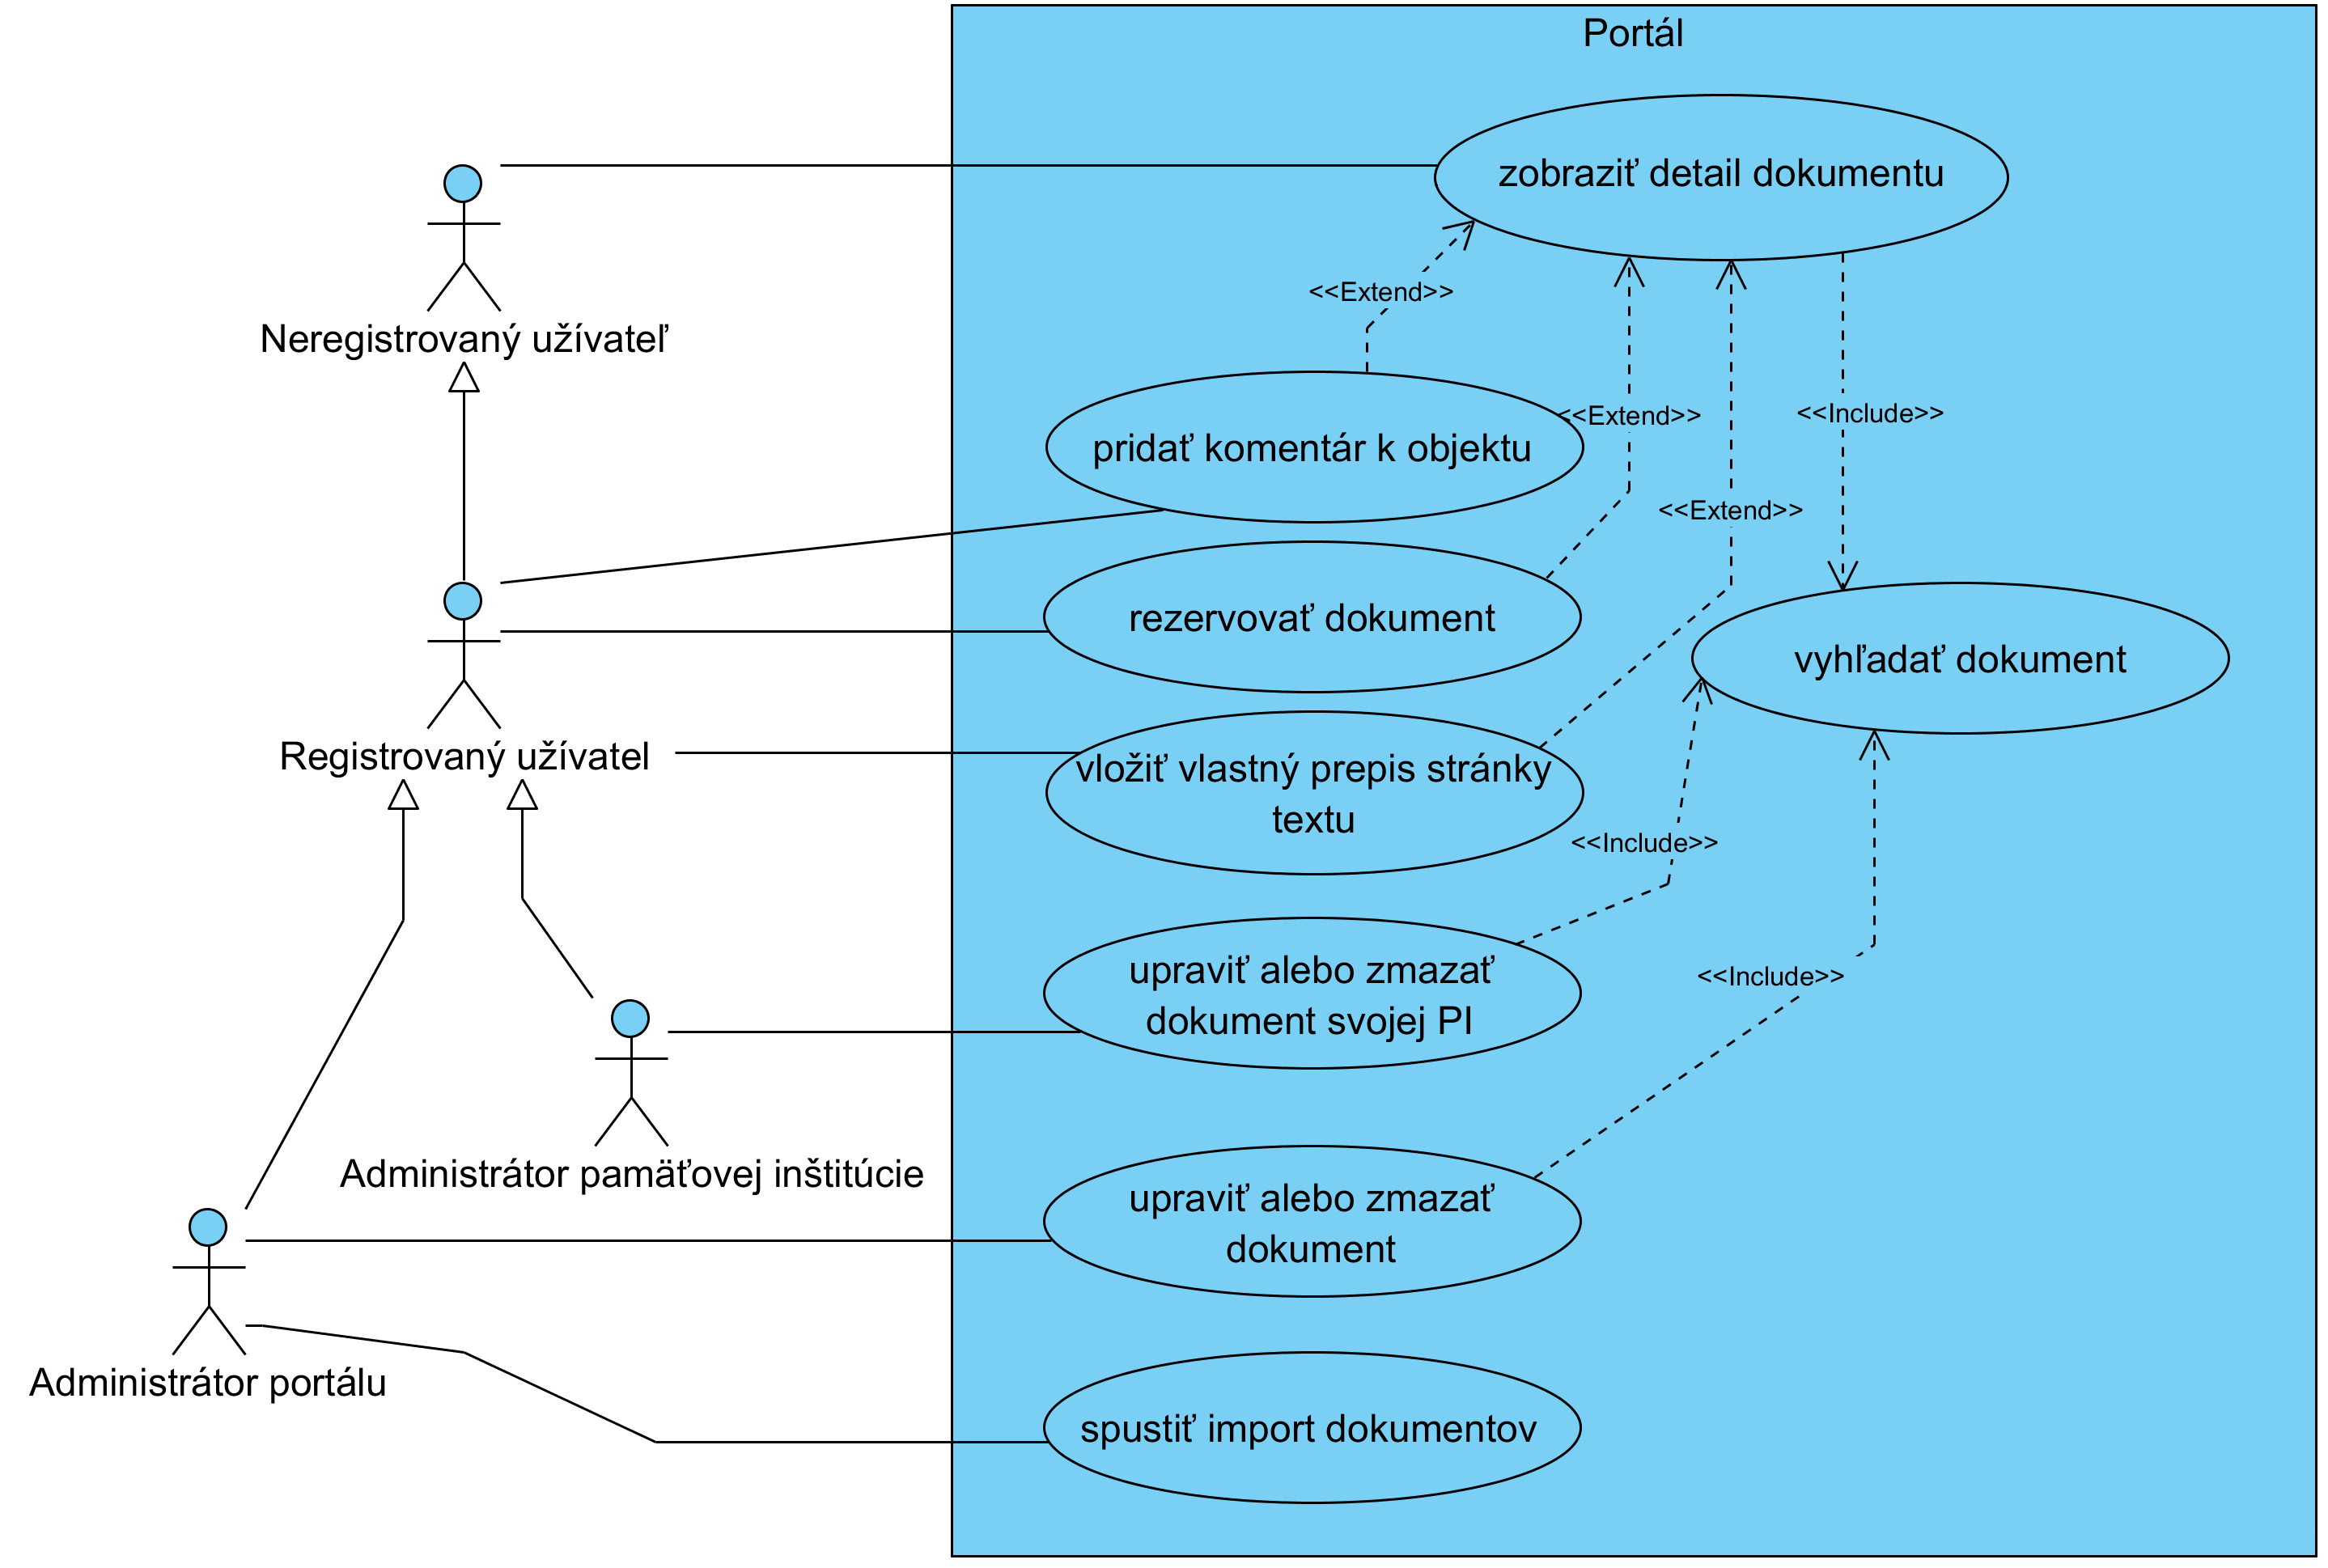
\includegraphics[width=\textwidth]{fithesis/diagram/useCase.png}
	
	\caption{Prípady použitia PD}
	\label{useCaseDG}
\end{figure}

\subsection{Kategórie dokumentov}
Dokumenty, ktoré sú predmetom prípravy a zverejnenia prostredníctvom portálu digitálneho kultúrneho dedičstva (ďalej už len PD) sú rozdelené do dvoch základných kategórií:
\begin{itemize}
	\item dokumenty archívnych fondov a múzejných zbierok				
	\item dokumenty knižničných fondov podľa štandardov NDK\footnote{NDK - Národní digitální knihovna}
\end{itemize}
Pre vyššie uvedené jednotlivé kategórie je nutné použiť v PD rozdielne pracovné postupy a to hlavne v prípravnej fáze pred zverejnením. Dôvodom je samotná podstata dokumentu z pohľadu toho, či ide o dokumenty, ktoré sú v nemennej podobe (monografie, periodiká) alebo dokumenty, u ktorých sa v čase môžu meniť predovšetkým ich popisné informácie. Pre každú kategóriu sú taktiež definované odlišné dátové štruktúry metadát. Predpokladaný objem dokumentov spravovaných PD je 100 000 jednotlivých dokumentov, 1 500 000 strán prepočítaných na formát A4 a približne 20 terabajtov obrazových dát.
\subsection{Dokumenty archívnych fondov a múzejných zbierok}
Druhy dokumentov:
\begin{itemize}
	\item fotografie, negatívy				
	\item zväzky - kroniky, zápisy, katalógy
	\item voľné archy - dokumenty, plagáty, plány
	\item staré výtlačky, spevníky
	\item kartografický materiál 
	\item filmy, zvukové nahrávky 
	\item zbierkové predmety	
\end{itemize}
Jedná sa o dokumenty, ktoré vznikli digitalizáciou vybraných archívnych fondov a múzejných zbierok. Z hľadiska nemennosti týchto dokumentov sa jedná o dokumenty premenlivej povahy. Popisné metadáta z KDJ\footnote{KDJ - Krajská digitalizační jednotka} pre PD u tejto kategórie preto nie je možné použiť. Jedná se teda o dokumenty, u ktorých je nutné ručné doplnenie metadát. 

\subsection{Dokumenty knižničných fondov podľa štandardov NDK}
Druhy dokumentov:
\begin{itemize}
	\item monografie - jednodielne alebo viacdielne knižné dokumenty			
	\item periodiká - pravidelne vychádzajúce výtlačky
\end{itemize}
Jedná sa o dokumenty prevažne nemennej povahy. Predpokladá se teda, že ako uložené digitálne obrazy, tak metadáta majú konečný a nemenný stav. Všetky tieto dokumenty sú uložené v úložisku KDJ vo formáte SIP. KDJ bude pre tento typ dokumentov zdrojovým poskytovateľom informácií pre PD. 
\subsection{Typy dokumentov} 
Z hľadiska typu súborov, v ktorých sú digitálne dokumenty uložené, se jedná o dokumenty:
\begin{itemize}
	\item obrazové			
	\item videá
	\item zvukové záznamy
	\item vo formáte XML (popisné metadáta)		
	\item vo formáte PDF
\end{itemize}
\subsection{Vstup dokumentov} 
Táto časť PD bude zabezpečovať riadený import dát pre prípravu sprístupnenia dokumentov. Vstupné mechanizmy budú rešpektovať potreby jednotlivých kategórií dokumentu. Po importe budú dáta pripravených dokumentov uložené do zverejňovacej databázy. Princíp predávania dokumentov, detailný popis rozhrania a jeho dátová štruktúra budú súčasťou implementačnej analýzy. Zákazník špecifikoval nasledujúce podmienky:
\begin{itemize}
	\item PD bude umožňovať import viacerých dokumentov súčasne.
	\item Pri zahájení prípravy vstupu dokumentu do PD bude prevedená kontrola duplicity s predchádzajúcimi importovanými dokumentmi.
	\item Behom importu dokumentu do PD systém priradí jeho vlastníka – osobu kompletne zodpovednú za celé sprístupnenie a zverejnenie. Vlastníkom se stáva užívateľ PD, ktorý import úspešne dokončil. Zdrojom dát pre import bude mimo iných webové rozhranie PD a zdieľané diskové zložky unikátne pre každého administrátora.
	\item PD bude disponovať funkciou pre import a aktualizáciu popisných metadát a prípadných obrazových dát zo systému JANUS2000 (evidenčný systém okresných archívov) a systému VISMO (dáta projektu \textit{MG on-line}).
\end{itemize}
\subsection{Príprava dokumentov k sprístupneniu}
Táto časť PD bude zahŕňať proces sprístupnenia dokumentov a možnosť ich úpravy pred zverejním. Zákazník špecifikoval nasledujúce funkcie:
\begin{itemize}
	\item PD po prihlásení do časti pre prípravu dokumentu ponúkne oprávnenému užívateľovi zoznam všetkých jeho dokumentov s informáciou o ich stave a možnosťou zverejnenia dokumentu pre všetkých užívateľov.
	\item PD umožní oprávnenému užívateľovi zobraziť náhľad upraveného dokumentu, znázorňujúci stav, v ktorom bude dokument zverejnený.
	\item PD umožňuje oprávnenému užívateľovi kedykoľvek zrušiť zverejnenie dokumentu. 
	\item Oprávnený užívateľ, vlastník dokumentu, má na karte otvoreného dokumentu k dispozícii históriu úprav.
	\item Portál PD umožní oprávnenému užívateľovi možnosť úpravy popisných dát podľa úrovne jeho oprávnení.
	\item Štruktúra dokumentu bude navrhnutá podľa štandardu Dublin Core.
	\item Všetky dôležité akcie PD ako sprístupnenie, úprava alebo zmazanie dokumentu budú sprevádzané notifikačným e-mailom pre všetkých dotknutých užívateľov.
\end{itemize}
\subsection{Operácie nad zverejnenými dokumentmi}
Táto časť portálu obsahuje funkcie dostupné pre širokú verejnosť, tzn. registrovaných a neregistrovaných užívateľov. Zákazník špecifikoval nasledujúce funkcie, dostupné všetkým užívateľom:
\begin{itemize}
	\item PD bude poskytovať možnosť vyhľadávania v celom texte.
	\item PD bude poskytovať možnosť vyhľadávania podľa konkrétnych atribútov.
	\item PD umožní export obsahu príslušného dokumentu do PDF súboru.
\end{itemize}
Nasledujúce funkcie budú dostupné všetkým registrovaným užívateľom:
\begin{itemize}
	\item Možnosti pre užívateľský popis príslušného dokumentu. Ide o diskusiu k dielu a prepis nerozpoznaného textu dokumentu.
	\item PD umožní rezerváciu diela pre vypožičanie.
\end{itemize}
\section{Návrh riešenia}
Na základe analýzy existujúcich nástrojov na prehliadanie digitálnych fondov a komunikácie so zákazníkom bol vytvorený konečný návrh projektu. Pre implementáciu PD bude využité open source
portálové riešenie \textit{Liferay} vo verzii \textit{6.2.2 community edition GA3}. Prípadný prechod na vyššiu verziu je možný prostredníctvom štandardných postupov pre portál Liferay a nieje zahrnutý v rozsahu tohto projektu. Zaznamenávanie operácií v PD bude zabezpečené pomocou frameworku pre Java aplikácie \textit{Log4j}. Výstupné hlášky sú štandardne zaznamenávané do súboru na aplikačnom serveri, na ktorom aplikácia beží. Jednotlivé hlášky budú rozdelené do úrovní. Nastavovanie týchto úrovní bude možné prostredníctvom administračného rozhrania portálu Liferay. Administrácia zverejňovania digitálneho obsahu bude dostupná všetkým oprávneným užívateľom. Vyhľadávanie bude dostupné všetkým užívateľom bez ohľadu na ich identitu.\cite{enterprise-systems}

\subsection{Grafický vzhľad}
Grafický vzhľad aplikácie bude meniteľný pomocou špeciálnych zásuvných modulov podporovaných portálom Liferay (tzv. témy). Téma bude využitá naprieč všetkými časťami portálu. Tento prístup zabezpečuje jednotný dizajn aplikácie. Zmena vzhľadu vyžaduje vývoj alebo úpravu zásuvného modulu.
\subsection{Komunikácia s externými systémami}
Pre komunikáciu s externými systémami budú použité následujúce technológie:
\begin{itemize} 
\item \textit{Protokol Z39.50} – pre komunikáciu s pamäťovými inštitúciami kvôli aktualizácii metadát dokumentov
\item \textit{Protokol OAI-PMH} – pre poskytnutie rozhrania, na zbieranie metadát v databáze externými aplikáciami
\end{itemize}
\subsection{Digitálny objekt}
Digitálny objekt je štruktúra, ktorá vstupuje na vonkajšom rozhraní PD do importovacej dávky. Táto štruktúra bude v priebehu importovacieho procesu spracovaná a transformovaná do vnútornej štruktúry PD.
Načítané digitálne objekty budú na základe svojich vlastností a zdrojových systémov delené do niekoľkých podskupín. Na delenie typov je možné nahliadať z dvoch rôznych perspektív.
\begin{itemize}
\item	Z pohľadu štruktúry dát 
\item	Z pohľadu vlastného obsahu digitálneho objektu
\end{itemize}
Digitálne objekty importované zo systému SIRIUS sú fyzicky reprezentované pomocou SIP balíčkov. A práve tieto SIP balíčky odpovedajú v prípade systému SIRIUS jednotlivým typom objektov vnútornej štruktúry dát PD.
\begin{figure}[H]
	\centering
		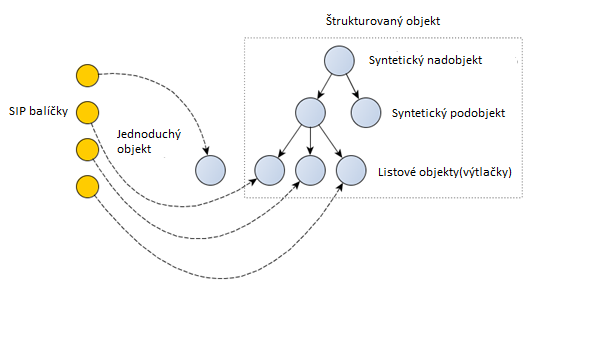
\includegraphics[width=\textwidth]{fithesis/obr/struktObj.png}
	
	\caption{Príklad štrukturovaného dokumentu s tromi úrovňami}
	\label{structDg3l}
\end{figure}
\subsection{Typy objektov z hľadiska štruktúry}
Jeden SIP balíček bude transformovaný do práve jedného listového objektu (v prípade štrukturovaného objektu) alebo do jedného jednoduchého objektu. Napríklad v prípade monografie je to priamo vlastný digitálny objekt. V prípade periodika je SIP balíček listový objekt, ktorý sa stane súčasťou štrukturovaného objektu a bude zaradený ako digitálny objekt na jeho najnižšej úrovni.
Z dát v listových objektoch bude možné zložiť celú štruktúru hierarchického digitálneho objektu pretože každý SIP balíček nesie informácie o celom štrukturovanom objekte a je možné príslušný objekt z týchto informácií vytvoriť. Dáta štrukturovaného objektu sú teda uložené redundantne v niekoľkých listových objektoch.
Či sa jedná o jednoduchý objekt alebo sa jedná o štrukturovaný objekt a typ dokumentu z pohľadu obsahu bude určovať algoritmus rozoznania typu objektu. 
\subsubsection{Jednoduchý objekt}
Jednoduchý objekt znamená, že v portáli budú uložené dáta o danom digitálnom objekte bez možnosti jeho prechádzania po úrovniach. V tomto prípade môžeme jeden digitálny objekt označiť za ekvivalent jedného SIP balíčku.
Z pohľadu obsahu sa jedná o nasledujúce typy:
\begin{itemize}
	\item Monografia
	\item Zbierkový predmet
	\item Rukopis
	\item Veduta
\end{itemize}
\subsubsection{Hierarchický objekt}
Hierarchický alebo štrukturovaný objekt je na najnižšej úrovni zložený z listových objektov a ďalších syntetických objektov. Jednotlivé úrovne ako aj vlastný koreňový objekt bude vždy možné identifikovať zo všetkých listových objektov. Z pohľadu obsahu se jedná o nasledujúce typy:
\begin{itemize}
\item Dvojúrovňové objekty
	\begin{itemize}
	\item Viaczväzková monografia
	\item Kronika
	\item Fotografia	
	\item Mapa
	\item Listina
	\end{itemize}
\item Trojúrovňové objekty
	\begin{itemize}
	\item Periodikum
	\item Úradný zápis	
	\end{itemize}
\end{itemize}
\subsubsection{Listový objekt}	
Listový objekt je základným stavebným prvkom štrukturovaného objektu. Na rozdiel od jednoduchého objektu je vždy sprevádzaný svojim syntetickým nadobjektom. Tento syntetický nadobjekt je vždy čitateľný zo všetkých SIP balíčkov, ktoré sú uložené do objektu na najnižšej úrovni. Pokiaľ bude v štrukturovanom objekte iba jeden listový objekt, bude ho portál stále zobrazovať ako viacúrovňový objekt.
\subsection{Typy objektov z hľadiska obsahu}
Z hľadiska obsahu objektov rozoznávame niekoľko typov. U jednotlivých typov obsahu je vždy potrebné rozhodnúť aké atribúty budú načítané zo SIP balíčkov do vnútornej štruktúry PD. Všetky relevantné atribúty budú zanesené do vyhľadávacieho indexu.

Pre jednoznačné odlíšenie digitálnych objektov budú využité atribúty generované systémom SIRIUS, ktoré budú zaisťovať ich jedinečnosť. Tieto atribúty môžu byť v závislosti od jednotlivých typov objektov rôzne. Podľa identifikátoru môžeme dokumenty rozdeliť do nasledujúcich skupín:
\begin{itemize}
	\item Parameter \textit{ČČNB} - monografie, viaczväzkové monografie, periodiká
	\item Parameter \textit{DIGIKUJIF} - fotografie
	\item Parameter \textit{DIGIKUJIM} - mapy
	\item Parameter \textit{DIGIKUJIK} - kroniky
	\item Parameter \textit{DIGIKUJIL} - listiny
	\item Parameter \textit{DIGIKUJIR} - rukopisy
	\item Parameter	\textit{DIGIKUJIV} - veduty
	\item Parameter \textit{DIGIKUJIZ} - úradné zápisy
\end{itemize}
\subsection{Návrh dizajnu}
Táto kapitola popisuje dizajn aplikácie a funkcie dostupné užívateľovi v jednotlivých sekciách.	Pre lepšiu predstavu, ako bude popisovaná funkcionalita vyzerať vo výslednom systéme, je pri prípadoch použitia uvedený nákres užívateľského rozhrania (tzv. mockup).
\subsubsection{Úvodná stránka portálu}
Úvodná stránka PD bude obsahovať čo najmenej informácií v záujme čo najväčšej prehľadnosti a jednoduchosti pre užívateľa. Konkrétne bude obsahovať:
\begin{itemize}
	\item vyhľadávací formulár
	\item najčastejšie hľadané objekty
	\item odkaz na kontaktné údaje
	\item odkaz na informácie o jednotlivých pamäťových inštitúciách
	\item odkaz na autorizované operácie pre prihláseného užívateľa
	\item mapu umiestnenia dokumentov
\end{itemize}
\begin{figure}[H]
	\centering
		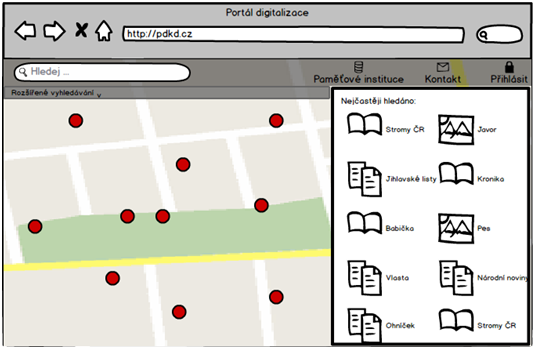
\includegraphics[width=\textwidth]{fithesis/mockup/welcome.png}	
	\caption{Nákres úvodnej stránky}
	\label{mockup-welcome}
\end{figure}
\clearpage

\subsubsection{Stručný detail objektu}
Stručný detail objektu sa zobrazí pri kliknutí na konkrétny vyhľadaný objekt. Stručný detail nebude zobrazený cez celú plochu okna prehliadača, ale iba na polovici okna. Druhá polovica bude obsahovať mapu s bodmi predstavujúcimi miesta vydania, uloženia, či miesta, ku ktorým sa objekt obsahovo vzťahuje. 

\begin{figure}[H]
	\centering
	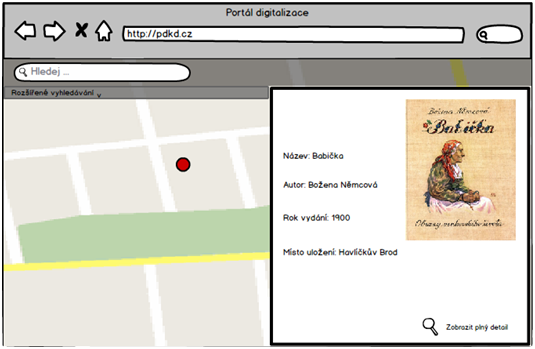
\includegraphics[width=\textwidth]{fithesis/mockup/detail-small.png}	
	\caption{Nákres stručného detailu objektu}
	\label{mockup-detail-small}
\end{figure}
\clearpage
\subsubsection{Plný detail objektu}
Úplný detail objektu sa zobrazí po kliknutí na tlačidlo \textit{Zobraziť plný detail} v stručnom detaile objektu. Plný detail bude zobrazený cez celú plochu okna prehliadača a bude zobrazovať všetky informácie o danom objekte.
Z plného detailu bude možné tento detail vytlačiť a exportovať do PDF. Rovnako bude možné vytlačiť a exportovať do PDF samotný objekt. Plný detail bude zobrazený na adrese, ktorá bude vo formáte permalinku. To znamená, že pri skopírovaní adresy z adresného riadku prehliadača do nového okna, bude zobrazený ten istý detail pôvodne zobrazeného objektu. Plný detail objektu bude tiež obsahovať napojenie na štandardné Facebook API, umožňujúce zdieľanie stránky.
\begin{figure}[H]
	\centering
	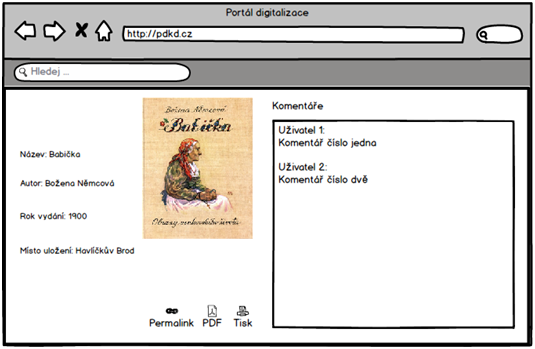
\includegraphics[width=\textwidth]{fithesis/mockup/detail-full.png}	
	\caption{Nákres plného detailu objektu}
	\label{mockup-detail-full}
\end{figure}
\clearpage
\subsubsection{Rozhranie pre import dát zo systému Sirius a Vismo}
V príslušnej aplikácii v administračnom rozhraní užívateľ klikne na tlačidlo \textit{Spustit} pri položke \textit{SIRIUS} alebo \textit{VISMO}. Import je zahájený a do výpisu v spodnej časti obrazovky sa vypisujú informácie o prebiehajúcom importe.
\begin{figure}[H]
	\centering
		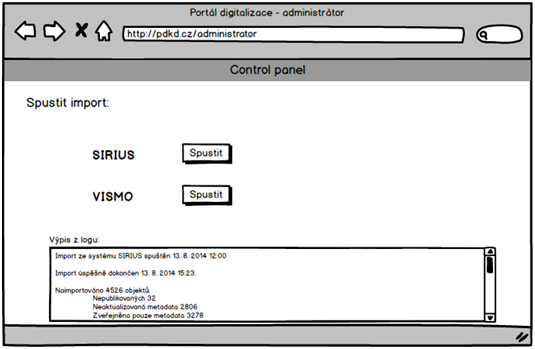
\includegraphics[width=\textwidth]{fithesis/mockup/import.png}	
	\caption{Nákres administračného rozhrania pre import dokumentov}
	\label{mockup-import}
\end{figure}
\clearpage
\subsubsection{Správa pamäťových inštitúcií}
Oprávnený užívateľ bude mať možnosť v administračnom rozhraní vytvárať, upravovať a mazať pamäťové inštitúcie so všetkými ich údajmi.
\begin{figure}[H]
	\centering
		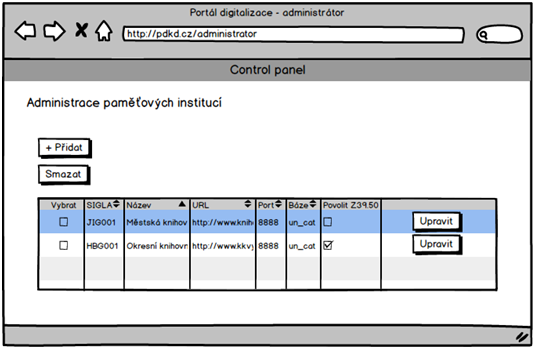
\includegraphics[width=\textwidth]{fithesis/mockup/institution.png}	
	\caption{Nákres rozhrania pre správu inštitúcií}
	\label{mockup-institution}
\end{figure}
\clearpage
\chapter{Technológie}
\section{Indexácia}
\subsection{Výber vyhľadávacieho nástroja}
Pre potreby indexácie boli v analytickej fáze zvažované tieto možnosti:
\begin{itemize}
	\item \textit{Elastic} – vyhľadávací nástroj postavený na Java knižnici \textit{Apache Lucene}
	\item \textit{Sphinx} – vyhľadávací nástroj vytvorený v jazyku C++
\end{itemize}
Po konzultácii s vývojovým tímom sa nakoniec rozhodlo pre \textit{Elastic} z dôvodu vyššej spoľahlivosti a jednoduchého používania.
\subsection{Elastic}
Elastic je nástroj na indexáciu dát. Jeho primárnym účelom je vyhľadávanie nad relatívne veľkým množstvom textu. Oproti databáze ponúka oveľa rýchlejšiu odpoveď a rozvinutejšie možnosti štrukturovaného ukladania dát. 

Aplikácie využívajúce Elastic s ním komunikujú pomocou HTTP protokolu a dotazy ako  aj odpovede sú vo formáte JSON. Príklad dotazu na Elastic:


\begin{lstlisting}[language=json,firstnumber=1]
GET
{
"query" : {
	"term" : { "gender": "female" },
	"range" : {
		"age" : {
		"from" : 20,
		"to" : 30
		}
	} 
}}
	\end{lstlisting}
Tento dotaz vyhľadá všetky záznamy s uvedenými parametrami. \textit{Term} je označenie výrazu, ktorý vyžaduje presný obsah určitého atribútu. \textit{Range} vyhľadá všetky záznamy ktoré sa nachádzajú v určenom rozmedzí. V tomto prípade hľadáme ženu od 20 do 30 rokov. Odpoveďou na takýto dotaz by mohlo byť napríklad:
\begin{lstlisting}[language=json,firstnumber=1]
"hits":{
  "total" : 1, 
	"hits" : [
		  {"_index" : "pdkd",
		   "_type" : "person",
		   "_id" : "1",
		   "_source" : { 
			  "name" : "Kim", 
			  "age" : 22,
			  "gender" : "female" 
		  }
	} 
	]
}
\end{lstlisting}
Výsledkom dotazu je teda 1 záznam.\cite{elastic-reference} 
\subsection{Ďalšie možnosti vyhľadávania}							
\subsubsection{Radenie}
Poradie vrátených záznamov môže byť vytvorené na základe určitého atribútu, relevancie výsledku alebo kombinácie týchto faktorov.
\subsubsection{Score}
Ďalšou zaujímavou funkciou elasticu je \textit{relevance scoring}. Po tom čo získame zoznam vyhovujúcich záznamov, je potrebné ich zoradiť podľa relevancie. V prípade kombinovaného dotazu s logickými spojkami neobsahuje každý záznam všetky podmienky. Skóre relevancie sa počíta na základe troch faktorov:
\begin{compactenum}
	\item \textbf{Frekvencia výskytu hľadaného výrazu v zázname} - čím viac je v zázname zmienená, tým je záznam podstatnejší.
	\item \textbf{Inverzná frekvencia hľadaného výrazu} – relevancia výrazu sa znižuje v závislosti od množstva záznamov obsahujúcich tento výraz.
	\item \textbf{Rozsah atribútu , v ktorom bol výraz nájdený} – čím je obsah atribútu dlhší, tým je relevancia tohto výskytu nižšia
\end{compactenum}
\subsubsection{Aggregations}			
Výsledky vyhľadávania je niekedy potrebné zlučovať do skupín na základe určitého parametru. \textit{Elastic} ponúka funkciu \textit{Aggregations}. Pokiaľ je teda v dotaze špecifikovaný atribút, na základe ktorého sa majú záznamy zoskupovať, je výsledkom objekt obsahujúci niekoľko skupín ďalších objektov, ktoré môžu predstavovať samotné záznamy alebo ďalšie skupiny zjednotení. Vďaka formátu JSON je možné tieto objekty serializovať. V prípade objektových jazykov ako Java je potom jednoduché poskladať štruktúry, s ktorými jazyk pracuje, pomocou knižnice na deserializáciu.  
\section{OAI-PMH}
OAI-PMH\footnote{OAI-PMH - The Open Archives Initiative Protocol for Metadata Harvesting} je protokol, ktorý sa používa na získavanie metadat elektronicky evidovaných dokumentov. Vznikol ako iniciatíva na zjednodušenie zbierania informácií vo viacerých separátnych repozitároch. Aj keď presný formát dát nie je určený, pre lepšiu interoperabilitu sa odporúča použitie štandardu Dublin Core.\cite{dublin-core} Pri použití protokolu sa na jednej strane komunikácie nachádza poskytovateľ, ktorý dáta vystavuje. Typicky ide o inštitúciu spravujúcu dané dokumenty. Záznamy sú do databázy poskytovateľa vkladané ručne alebo v prípade dokumentu vystaveného inou inštitúciou je možné proces automatizovať a použiť informácie získané z tohto zdroja. Záznamy môžu byť upravované a vykonané zmeny sa prejavia vo vystavených dátach. Na druhej strane je zberateľ, ktorý o dáta žiada. Pomocou protokolu môže zozbierať metadáta dokumentov z rôznych inštitúcií a vytvoriť rozhranie pre užívateľov, ktorí takto môžu vyhľadávať nad zjednotenými informáciami na jednom mieste.\cite{oai1},\cite{oai2}
\section{Z39.50}
Protokol Z39.50 je protokol na vyhľadávanie nad textovými databázami. Typicky sa využíva v knižničných systémoch. Na rozdiel od OAI-PMH nie je nutné dáta zozbierať a vytvoriť vyhľadávacie rozhranie, ale je možné vyhľadávať priamo nad databázou konkrétnej inštitúcie. Je tiež možné vytvoriť rozhranie pre jednoduchšie používanie, zjednotenie informácií z viacerých zdrojov alebo kombináciu s vyhľadávaním nad miestnou databázou. \cite{z39501},\cite{z39502}      
\section{Portál}
\subsection{Použitie portálu}
Z užívateľského pohľadu je portál webová stránka, ktorá slúži ako jednotný bod prístupu k informáciám. Zámerom portálu je vytvoriť vstupnú bránu pre užívateľa po pripojení na internet. Môže zoskupovať informácie z rôznych zdrojov a zobrazovať ich užívateľovi na jednom mieste. Portál sa automaticky prispôsobuje potrebám konkrétneho užívateľa, ktorý ho používa. Užívateľ by tiež mal mať možnosť prispôsobiť zobrazený obsah podľa svojich potrieb.\cite{portal-common1}
\subsection{Portálové technológie}
K zobrazovaniu zjednotených informácií používa portál portlety. Portlet je webová aplikácia, ktorá je zodpovedná za jednu alebo viac funkcií.  Portlety bývajú štandardne súčasťou portálu po inštalácii, pretože niektoré požiadavky na funkcionalitu sa opakujú. Týmto spôsobom je možné zabezpečiť prihlasovanie užívateľov, systém oprávnení alebo zobrazovanie jednoduchého obsahu bez potreby ďalšej implementácie.\cite{portal-common2}

Do portálu je tiež možné nasadiť vlastné portlety. Najnovšia špecifikácia popisujúca vývoj týchto portletov je JSR\footnote{JSR - Java Specification Request} 286, ktorá popisuje interakciu aplikácií s portálom. Vďaka tomu je možné vytvárať portlety, ktoré sú ľahko rozšíriteľné a prenositeľné bez ohľadu na typ použitej portálovej technológie.
\section{Databázový systém}
Z analýzy požiadavkov vyplýva, že aplikácia potrebuje pre svoj beh databázu, v ktorej budú uložené všetky dáta vytvorené samotnou aplikáciou. Ostatné informácie ako užívateľské údaje, rozloženie portletov na stránke alebo akékoľvek dáta generované existujúcimi aplikáciami portálu Liferay sú ukladané do oddelenej databázy. Obidve databázy sú v správe KDJ. Pre tento prípad sú vystavené dve inštancie databázovej technológie MSSQL.  
\section{Liferay Portal}
V analytickej fáze projektu boli zvažované viaceré portálové technológie ako napr. GateIn, Jetspeed a WebSphere. Nakoniec bola zvolená technológia Liferay Portal. Táto technológia vyniká výbornou dokumentáciou, celosvetovým počtom užívateľov a dostupnosťou. Liferay Portal je open source riešenie, ktoré je možné zakúpiť v troch úrovniach podpory alebo ho využívať bezplatne vo verzii CE\footnote{CE - Community edition}. Od verzie 6 je liferay otvorený pod licenciou LGPL, ktorá garantuje prístup ku zdrojovým kódom počas implementácie. Táto vlastnosť v kombinácií s možnosťou nahradenia existujúcich modulov z neho robí vysoko prispôsobiteľnú vývojovú platformu\cite{yuan-interface},\cite{yuan-build}.
\clearpage
\begin{figure}[H]
	\centering
		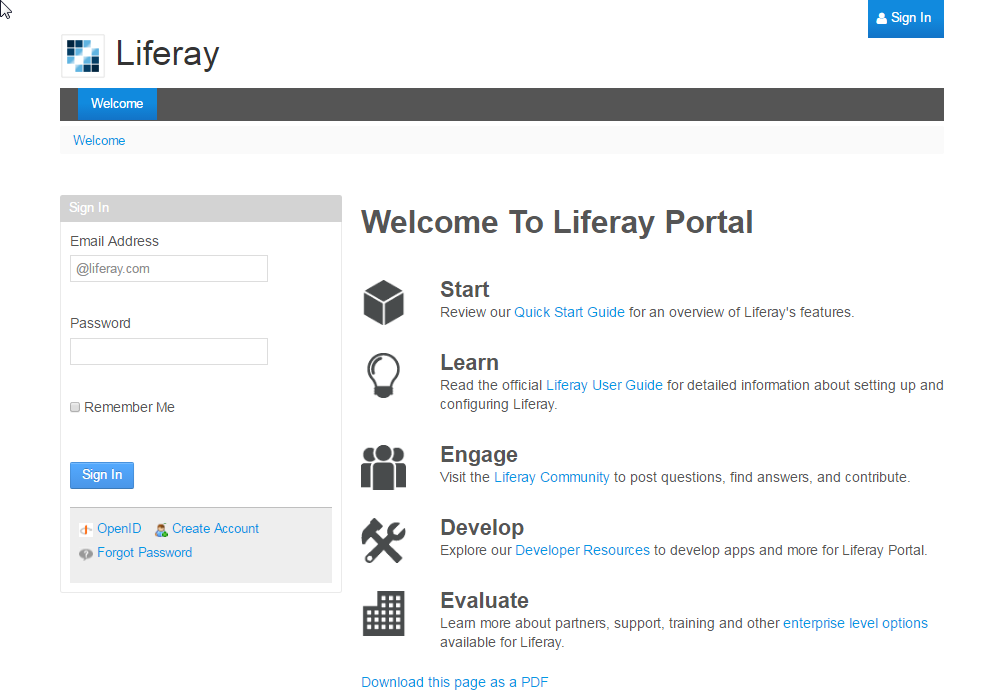
\includegraphics[width=\textwidth]{fithesis/obr/liferayUvod.png}	
	\caption{Práve nainštalovaný Liferay Portal}
	\label{liferayUvod}
\end{figure}
\noindent Na obrázku \textit{3.1} je zobrazená úvodná stránka portálu bez akejkoľvek modifikácie. Obsahuje odkazy na prihlásenie, manuály na používanie portálu alebo integráciu s OpenID.
\chapter{Implementácia}
\section{Využité portlety Liferay Portal}
Pred implementáciou samotnej aplikácie bolo potrebné určiť, akú časť funkcionality poskytovanej technológiou Liferay Portal je možné použiť v PD. Rozhodli sme sa pre nasledujúce moduly:
\begin{itemize}
	\item \textit{Web Content Management Portlet} - obsahuje funkcie CMS\footnote{CMS - content management system}
	\item \textit{Message Boards Portlet} - umožňuje pridávanie diskusie k objektu na základe primárneho kľúča
	\item \textit{Asset Publisher Portlet} - umožňuje označovanie dokumentov pomocou tzv. štítkov, v PD je zodpovedný za žiadosti o rezervácie dokumentov
	\item \textit{Asset Publisher Portlet} - stará sa o evidenciu kľúčových operácií v portáli, administrátor ju môže zobraziť priamo zo správcovského rozhrania 
\end{itemize}
\section{Štruktúra aplikácie}
Obslužné triedy aplikácie sa delia do troch balíkov. Každý z nich je z pohľadu programovacieho jazyka Java samostatná knižnica. Ich funkcie sú nasledovné:
\begin{itemize}
	\item \textit{core} - balík zodpovedný za funkcionalitu na pozadí aplikácie, obsahuje entity predstavujúce záznamy v databáze, stará sa o všetky operácie nad databázou aplikácie, implementuje rozhrania z balíku \textit{interface} ale nie je na ňom závislá
	\item \textit{interface} - obsahuje objekty typu DTO\footnote{DTO - data transfer object}, predstavuje komunikáciou medzi frontend a backend, \textit{portlet} využíva operácie, kotré tento balík poskytuje, \textit{core} ich implementuje
	\item \textit{portlet} - balík zodpovedný za frontend funkcionalitu, obsluhuje požiadavky užívateľa, stará sa o zobrazovanie obsahu\cite{java-ee}
\end{itemize}
\section{Digitálny objekt}
Na začiatku implementácie bola vytvorená štruktúra digitálnych objektov. Na vrstve \textit{interface} je reprezentovaná týmito objektmi:
\begin{itemize}
	\item \textit{DigitalObjectDto} - abstraktná trieda, predstavuje spoločný základ pre všetky digitálne objekty, obsahuje základné atribúty ako napríklad \textit{id, miesto uloženia, názov}
	\item \textit{SiriusObjectDto} - abstraktná trieda, predstavuje základ pre všetky objekty okrem zbierkových predmetov, rozširuje triedu \textit{DigitalObjectDto} o nasledujúce atribúty:
	\begin{itemize}
		\item \textit{sigla} - identifikátor inštitúcie, ktorá vlastní objekt
		\item \textit{sipPackageName} - názov SIP balíčku, z ktorého bol záznam poskladaný
		\item \textit{PhysicalDescriptionDto} - samostatný objekt, v ktorom je uložený popis dokumentu a informácie o jeho vytvorení
	\end{itemize}
	\item \textit{MonographSingleDto} - reprezentuje monografiu, pridáva atribút \textit{ccnb} (číslo České národní bibliografie)
	\item \textit{MonographMultivolumeDto} - reprezentuje jeden výtlačok viaczväzkovej monografie, pridáva atribút \textit{partNumber}
	\item \textit{PeriodicalIssueDto} - reprezentuje jeden výtlačok periodika, pridáva atribút \textit{issueNumber} a \textit{subTitle}
	\item \textit{MapDto} - reprezentuje mapu, pridáva atribút \textit{scale} (mierka mapy)
	\item \textit{PhotographDto} - reprezentuje fotografiu, pridáva atribút \textit{imageNumber}
	\item \textit{OfficialRecordIssueDto} - reprezentuje úradný dokument
	\item \textit{VedutteDto}	
\end{itemize}
Pre prácu s digitálnymi objektmi a pomocnými triedami boli v balíku \textit{interface} vytvorené nasledujúce objekty:
\begin{itemize}
	\item \textit{DigitalObjectService} - vykonáva CRUD\footnote{CRUD - create, read, update, delete} operácie nad digitálnymi objektmi
	\item \textit{DigitalObjectConverter} - konvertuje entity na DTO a naopak
	\item \textit{PhysicalDescriptionService} - CRUD a konverzia popisov objektov
	\item \textit{LanguageService} - CRUD a konverzia nad \textit{LanguageDto}
	\item \textit{LocationService} - CRUD a konverzia nad \textit{LocationDto}
\end{itemize}
Tieto rozhrania sú implementované v balíku \textit{core}. Názvy tried sú tvorené z názvov rozhraní pridaním prípony \textit{Impl}.
\section{Controller}
\textit{Controller} je komponenta systému, ktorá obsluhuje prichádzajúce požiadavky užívateľa. Je súčasťou návrhového vzoru MVC\footnote{MVC - model-view-controller}. Z hľadiska funkcionality aplikácie PD predstavuje jeden logický celok. Nasledujúce triedy reprezentujú príslušné controllery:
\begin{itemize}
	\item \textit{DigitalObjectDetailViewController} - obsluhuje funkcie plného detailu digitálneho objektu
	\item \textit{DocumentReaderViewController} - obsluhuje funkcie vyhľadávania a mapy
	\item \textit{ImportAdminViewController} - obsluhuje funkcie rozhrania pre import
	\item \textit{InstitutionViewController} - obsluhuje funkcie rozhrania pre správu a výpis pamäťových inštitúcií	
\end{itemize}
\section{Príklad fungovania aplikácie}
Logiku aplikácie si môžeme najlepšie ukázať na jednoduchom príklade. Zvolíme si akcie a vstupné informácie.  Užívateľ sa nachádza v administrácii a má otvorený formulár na úpravu dokumentu v ktorom zmenil názov diela. Po kliknutí na tlačidlo \textit{Uložiť} vykoná aplikácia nasledujúce kroky:
\begin{compactenum}
	\item Na základe parametra \textit{ACTION\_DIGITAL\_OBJECT\_NAME} rozozná o aký typ akcie sa jedná a priradí hodnotu atribútu \textit{ADMINISTRATED\_DTO} v tele requestu do parametra \textit{digitalObjectDto} v metóde \textit{updateMonographSingleDocument()}.
	\item Skontroluje formulár. V prípade chyby zapíše výnimku do logu aplikácie a upovedomí užívateľa.
	\item V prípade akceptovateľného formulára zavolá metódu \textit{updateDigitalObject(digitalObjectDto)} v triede \textit{DigitalObjectManager}, ktorá vykoná nasledujúce kroky:
	\begin{compactenum}
		\item Pomocou konvertora digitálnych objektov získa z objektu typu \textit{Dto} entitu digitálneho objektu.
		\item Uloží zmenenú entitu do databázy na základe parametra \textit{id}.
		\item Upraví záznam vo vyhľadávacom indexe tak aby odpovedal databázovému záznamu.		
	\end{compactenum} 
	\item Nastaví hodnotu parametra \textit{PARAM\_PAGE} na \textit{PAGE\_EDIT\_DIGITAL\_OBJECT} a hodnotu parametra \textit{PARAM\_ID} na id upravovaného dokumentu, čím zabezpečí návrat na stránku úpravy dokumentu.	 
\end{compactenum}
\bigskip Nasledujúca ukážka kódu vykonáva funkcionalitu popísanú vyššie.
\begin{lstlisting}[language=Java, basicstyle=\small, style=java-nice]
@ActionMapping(ACTION_DIGITAL_OBJECT_SAVE)
public void updateMonographSingleDocument(Model model, 
   ActionRequest request, ActionResponse response,
@Valid @ModelAttribute(ADMINISTRATED_DTO) DigitalObjectDto 
   digitalObjectDto, BindingResult result) {

   if (!result.hasErrors()) {
      sendMetadataEditedEmails(digitalObjectDto.getId());
      digitalObjectManager.updateDigitalObject(digitalObjectDto);
      SessionMessages.add(request, "digital-object-form-saved");
      LogMF.info(LOG, "Digital object ID: {0} updated successfully", 
         new Object[]{digitalObjectDto.getId()});
   } else {
      LogMF.error(LOG, "Error updating Monograph Single Document: {0}",
         new Object[]{result.getAllErrors()});
      SessionErrors.add(request, "monograph-form-contain-error");
   }
    
   response.setRenderParameter(PARAM_ID, 
      digitalObjectDto.getId());
   response.setRenderParameter(PARAM_PAGE, 
      PAGE_EDIT_DIGITAL_OBJECT);
 }
\end{lstlisting}


\chapter{Záver}
Ciele zvolené na začiatku práce sa podarilo naplniť. Vytvorili sme portál, ktorý spĺňa požiadavky popísané v analýze. Aktuálna verzia prešla testovaním a je nasadená na produkčnom serveri, ktorý je sprístupnený verejnosti.

Zvolený spôsob digitalizácie dát sa ukázal ako vhodný. Ako dobrá voľba sa tiež ukázala mapa, ktorá dodala portálu vysokú mieru prehľadnosti a robustná platforma \textit{Liferay Portal}, vďaka ktorej bolo možné implementovať dodatočné požiadavky zákazníka spoľahlivo a rýchlo.

Za zmienku stojí aj fakt, že celé riešenie aplikácie využíva open source technológie, za ktorými ale stojí široká vývojárska komunita. Touto cestou sme boli schopní postaviť robustné, spoľahlivé a zároveň lacné riešenie bez použitia platenej verzie \textit{Liferay Portal} alebo zvažovanej technológie \textit{SharePoint}.

Po nasadení portálu do ostrej prevádzky sa ponúkajú ďalšie možnosti rozvoja portálov kultúrneho dedičstva. Pre toto riešenie sa zatiaľ rozhodol len jeden kraj Českej republiky. Ak by ich postupne pribudlo viac, bolo by oveľa jednoduchšie zdieľať dáta medzi týmito inštitúciami, keďže jednou z najväčších prekážok pre digitalizáciu je nejednotný formát dát a zverejňovacích rozhraní. Týmto spôsobom by tiež bolo možné evidovať nehnuteľnosti alebo historicky významné miesta. Portálové riešenie ale nie je obmedzené len na kultúrne dedičstvo a časom by sa mohlo pristúpiť k evidencii prírodopisných zbierok, minerálov, živočíchov ale aj prírodných útvarov a pamiatok. Vzhľadom k tomu, že mapová nadstavba je už súčasťou riešenia, nie je ťažké si v budúcnosti predstaviť využitie portálu na plánovanie náučnej trasy po okresoch Českej republiky.  
\chapter*{Literatúra}
\printbibliography[heading=none] %% Print the bibliography.
\chapter*{Prílohy}
Súčasťou práce sú aj nasledujúce prílohy:
\begin{itemize}
	\item Diagram tried PD
\end{itemize}
\end{document}
